\documentclass{article}

\usepackage[table]{xcolor}    % loads also colortbl
\usepackage{tabularx}
\usepackage{color}
\usepackage{geometry}
\usepackage{hyperref}
\usepackage{graphicx}
\usepackage{longtable}
\usepackage{changepage}
\usepackage{hyperref}

% A4 is 210mm × 297mm
\geometry{
	a4paper,
	total={194mm, 289mm},
	left=3mm,
	top=4mm,
}

\definecolor{background}{rgb}{0.824,0.918,0.945}
\definecolor{border}{rgb}{0.282,0.675,0.776}

\renewcommand{\familydefault}{\sfdefault}
% https://tex.stackexchange.com/a/150650
\newcommand{\tabitem}{~~\llap{\textbullet}~~}
% https://tex.stackexchange.com/a/89932
\newcolumntype{Y}{>{\centering\arraybackslash}X}
% https://tex.stackexchange.com/a/343329
\renewcommand\tabularxcolumn[1]{m{#1}}% for vertical centering text in X column

\newcommand{\OngoingStatus}{\textcolor{red}{\textbf{Ongoing}}}
\newcommand{\Closed}[1]{\textcolor{black}{\textbf{Closed #1}}}

\begin{document}

\arrayrulecolor{border}
\arrayrulewidth=1pt

\rowcolors{2}{}{background}

\begin{tabularx}{\textwidth}{
    |>{\hsize=.47\hsize}X|
	>{\hsize=1.53\hsize}X|
}
\hline
\multicolumn{2}{|c|}{\textbf{Software Engineering Design 2019 Group 2 Meeting Minutes}} \\
\hline
Date & 2019/10/22 \\
\hline
Time & 20:00 - 22:30 \\
\hline
Location & CSIE building room 544 \\
\hline
Facilitator & Chih-Hsuan Yen \\
\hline
Recorded by & Yifan Wu \\
\hline
Objective & Decide on how to breakdown web2py \\
\hline
\end{tabularx}

\rowcolors{2}{background}{}
\vspace{-1mm}
\begin{tabularx}{\textwidth}{|X|X|X|X|}
\hline
\multicolumn{4}{|c|}{\textbf{Participants}} \\
\hline
Name & E-mail & Role & Present or not \\
\hline
Chih-Hsuan Yen & yan12125@gmail.com & Team Leader & Y \\
\hline
Chen-Hung Wu & ac791228@gmail.com & Team Member & Y \\
\hline
Po-Sheng Lin & b890052@gmail.com  & Team Member & Y \\
\hline
Cheng-Jhih Shih & cs861324@gmail.com & Team Member & Y \\
\hline
Jui-Che Wu & ss900405twtw@gmail.com & Team Member & Y \\
\hline
Yifan Wu &  eurekalilychou@gmail.com & Team Member & Y \\
\hline
Pin-Yen Huang & pinyentraffic@gmail.com & Team Member & Y \\
\hline
Wei-Jie Liang & jack55513608@gmail.com & Team Member & Y \\
\hline
\end{tabularx}

\vspace{-1mm}
\rowcolors{2}{background}{}
\begin{tabularx}{\textwidth}{|X|}
\hline
\multicolumn{1}{|c|}{\textbf{Meeting Agenda}} \\
\hline
	\begin{itemize}
		\item Discuss homework and draw class diagram together
	\end{itemize} \\
\hline
\end{tabularx}

\rowcolors{2}{}{}
\begin{longtable}{|p{\textwidth}|}
\hline
\rowcolor{background}
\begin{center}
\vspace{-1.5em}\textbf{Issues}\vspace{-1em}
\end{center} \\
\hline
\endhead

\begin{itemize}
    \item Assign codes to team members
    \begin{itemize}
	    \item Two stages: core modules first, then extensions and addons
	    \item Split the web framework into multiple parts by functionality \href{https://hackmd.io/Rbfyifz7SAGPlYIHPAoaKg?view#\%E5\%88\%86\%E9\%A1\%9E}{HackMD document}
	    \item according to personal preference
	\end{itemize}
    \item References
    \begin{itemize}
        \item \href{https://github.com/web2py/web2py/}{Github}
        \item \href{http://www.web2py.com/}{Official website}
        \item \href{http://www.web2py.com/books/default/chapter/29/00/preface}{Tutorial}
        \item \href{https://mdipierro.github.io/web2py/web2py_manual_5th.pdf}{Complete reference manual}
    \end{itemize}			
	\item Discuss class diagram exercises
\end{itemize}

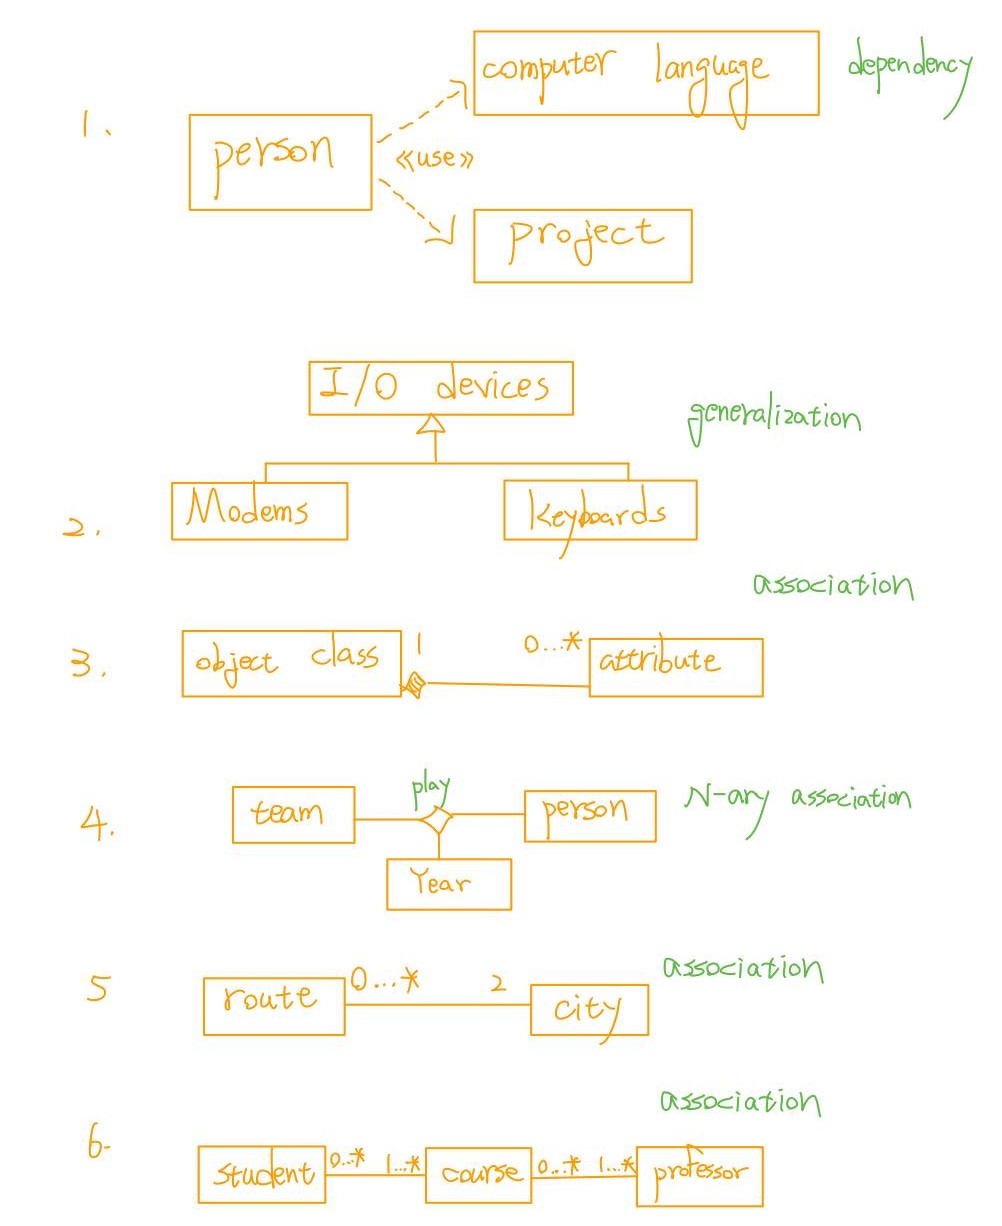
\includegraphics[scale=0.6]{class-diagram-1}
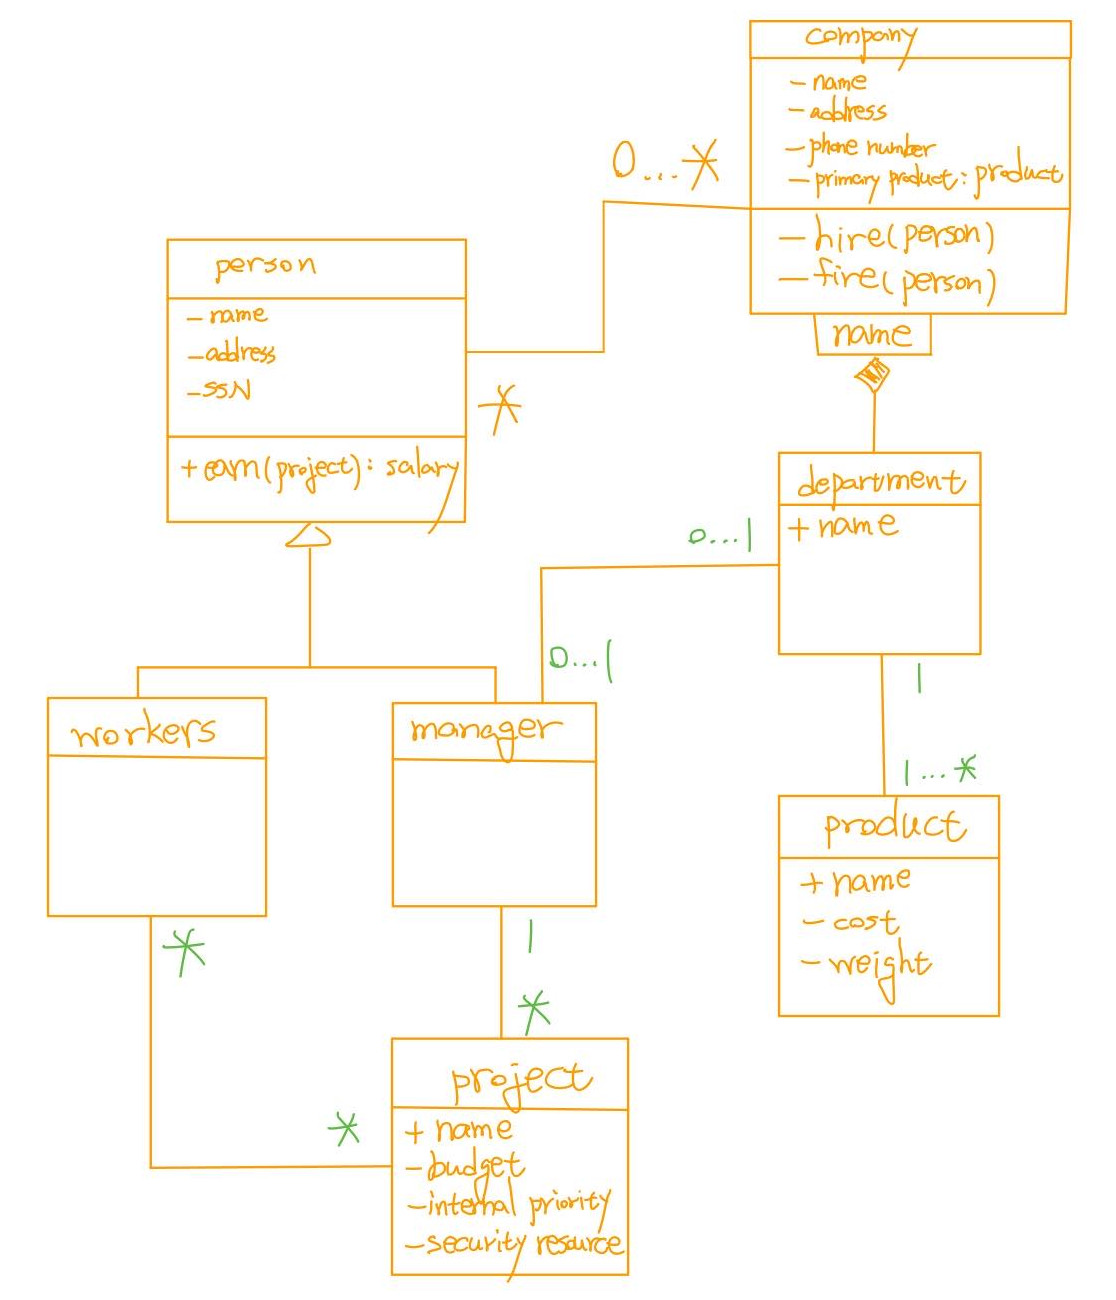
\includegraphics[scale=0.5]{class-diagram-4}
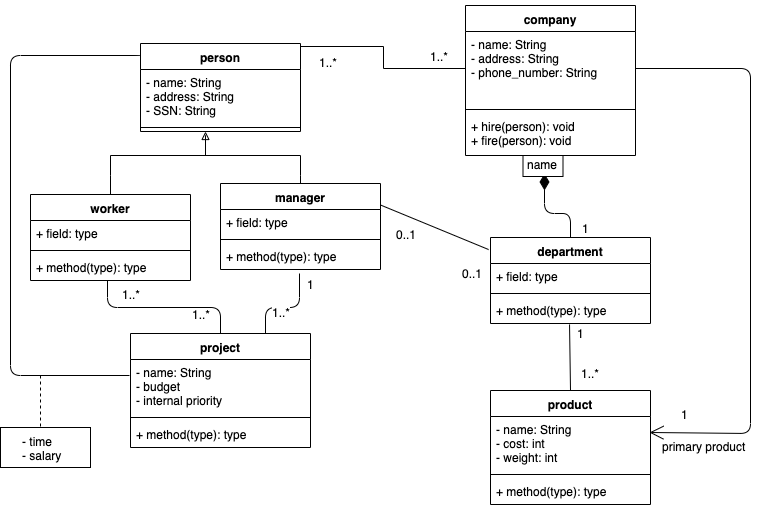
\includegraphics[scale=1.4]{class-diagram-2} \\
\hline
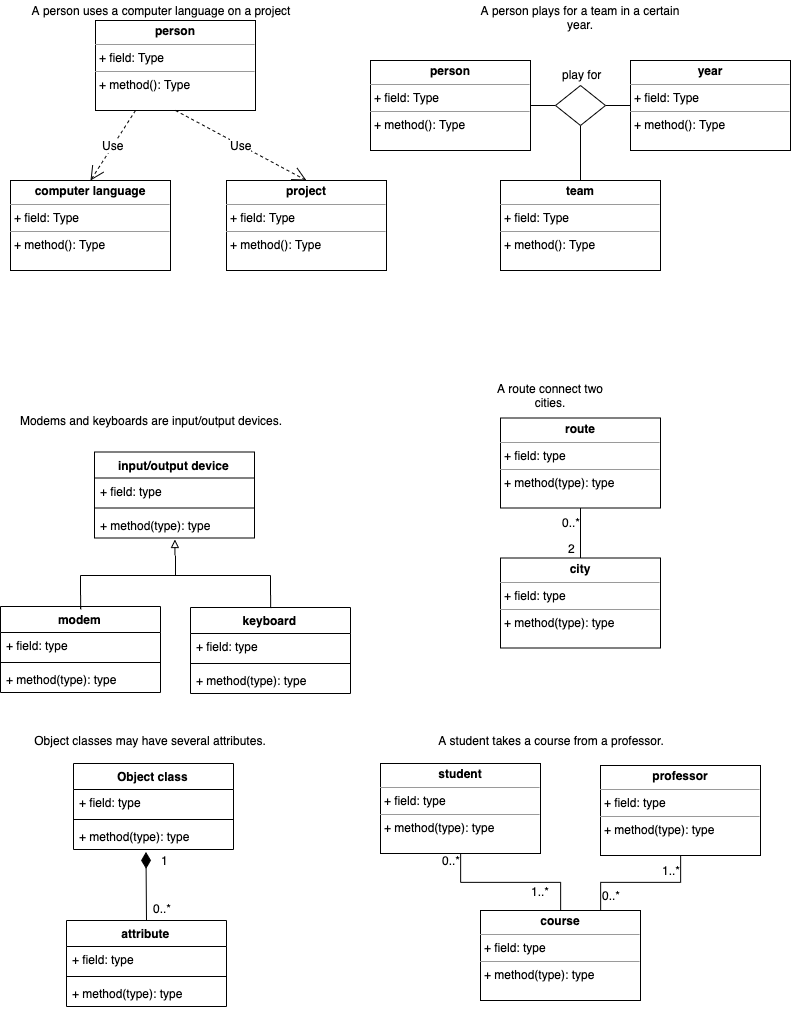
\includegraphics[scale=0.5]{class-diagram-3} \\
\hline
\end{longtable}

\rowcolors{2}{}{background}
\vspace{-1mm}
\begin{tabularx}{\textwidth}{
	|c|
	 >{\hsize=2\hsize}Y|
	 >{\hsize=.5\hsize}Y|
	 >{\hsize=.4\hsize}Y|
	 >{\hsize=.6\hsize}Y|
	 >{\hsize=.5\hsize}Y|
}
\hline
\multicolumn{6}{|c|}{\textbf{Action Items}} \\
\hline
No. & Action Items & Responsibility & Deadline & Status & Remark \\
\hline
1 & Survey Grails & Chih-Hsuan Yen, Yifan Wu & 10/1 & \Closed{10/1} & \\
\hline
2 & Survey Web2py & Po-Sheng Lin, Chen-Hung Wu & 10/1 & \Closed{10/1} & \\
\hline
3 & Survey DropWizard & Cheng-Jhih Shih, Pin-Yen Huang & 10/1 & \Closed{10/1} & \\
\hline
4 & Survey Nutch & Jui-Che Wu & 10/1 & \Closed{10/1} & \\
\hline
5 & Requests to responses & Billy, Yifan & 10/8 & \Closed{10/8} & \\
\hline
6 & How PyDAL works & WJ, WuCH, Jui-Che Wu & 10/8 & \Closed{10/8} & \\
\hline
7 & Overall structure & Chih-Hsuan Yen, Pin-Yen, Cheng-Jhih & 10/8 & \Closed{10/8} & \\
\hline
8 & Overall structure of PyDAL & WJ, WuCH, Jui-Che Wu & 10/15 & \Closed{10/15} & \\
\hline
9 & Function of gluon/*.py  & Pin-Yen  & 10/15 & \Closed{10/15} & \\

\hline

10 & Function of gluon/contrib/[a-o]*.py  & Chih-Hsuan Yen  & 10/15 & \Closed{10/15} & \\

\hline

11 & Function of gluon/contrib/[p-z]*.py  & Cheng-Jhih & 10/15 & \Closed{10/15} & \\

\hline

12 & scheduler.py & WuCH & 10/29 & \OngoingStatus & \\

\hline

13 & rocket.py & Po-Sheng Lin Pin-Yen & 10/29 & \OngoingStatus & \\

\hline

14 & rewrite.py & Cheng-Jhih &  10/29 & \OngoingStatus & \\

\hline

15 & widget.py & Jui-Che Wu &  10/29 & \OngoingStatus & \\

\hline

16 & sql.py & Wei-Jie Liang &  10/29 & \OngoingStatus & \\

\hline

17 & html.py & Chih-Hsuan Yen & 10/29 & \OngoingStatus & \\

\hline

18 & globals.py & Yifan Wu & 10/29 & \OngoingStatus & \\

\hline

\end{tabularx}

\end{document}
